\section{Introduction}

\subsection{History}

\begin{frame}
  \note{
    \begin{itemize}
    \item Present birth of AI: McCarthy, Dartmouth workshop, 1956
    \item Previous ideas
      \begin{itemize}
      \item Philosophy, logic, Turing machine, information theory, cybernetics
      \end{itemize}
    \item Birth of ML as a field of AI: Arthur Samuel, 1959
      \begin{itemize}
      \item Adaptation instead of explicit programming
      \end{itemize}
    \item Insist on broad approaches:
      \begin{itemize}
      \item symbolic \vs{} connexionist
      \item link with cognitive sciences
      \end{itemize}
    \item Concrete realizations:
      \begin{itemize}
      \item Modern programming languages: OO, more dynamic, CAS
      \item Problem solving: navigation on graphs
      \item Mc Carthy: as soon as it works, nobody calls it AI anymore
      \end{itemize}
    \item Over-optimistic preditions:
      \begin{itemize}
      \item Herbert Simon, 1958:  within ten years a digital computer will be
        the world's chess champiom
      \end{itemize}
    \end{itemize}
  }
  \frametitle{Birth \& early successes (1956--1973)}

  \begin{textblock}{100} (0,10)
    \begin{center}
      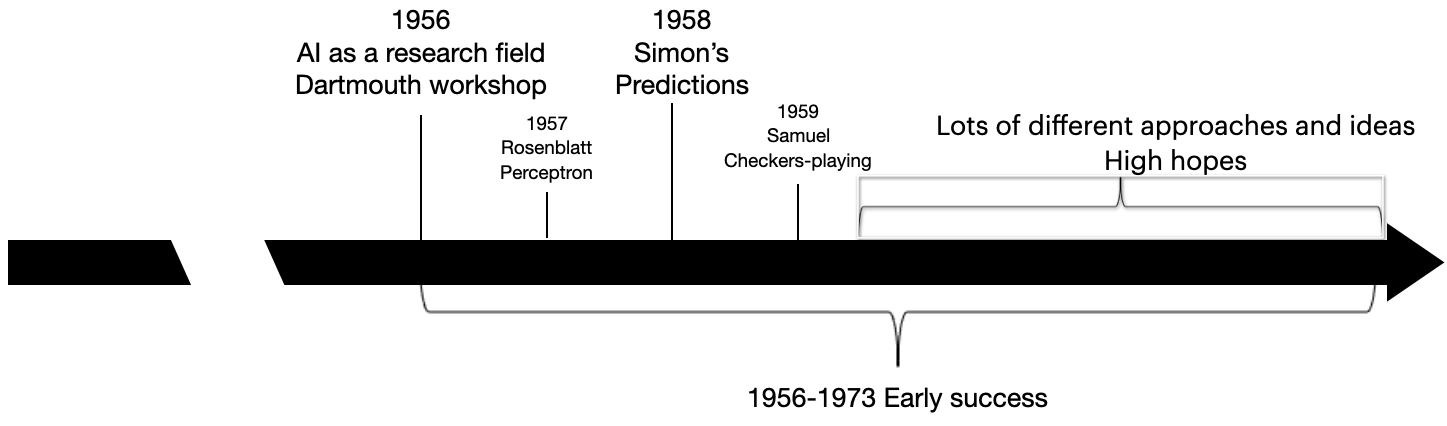
\includegraphics[width=0.95\textwidth]{img/ai_history_1956_1973.png}
    \end{center}
  \end{textblock}

  % Résumé de la frise
  \begin{textblock}{50}(0, 50)
    \begin{itemize}
      \item \aclu{AI} (1956)
        \begin{itemize}
        \item \footnotesize Discipline focused on creating systems capable of performing tasks that typically require human intelligence, such as learning, problem-solving and decision-making.
        \end{itemize}
      \item<2-> \acl{ML} (1959)
        \begin{itemize}
        \item \footnotesize Field of AI focused on the development and study of machines that can learn from data and generalize to unseen data.
        \end{itemize}
      \end{itemize}
    \end{textblock}

    % Résumé des réalisations
    \begin{textblock}{50}(50, 50)
      \begin{center}
        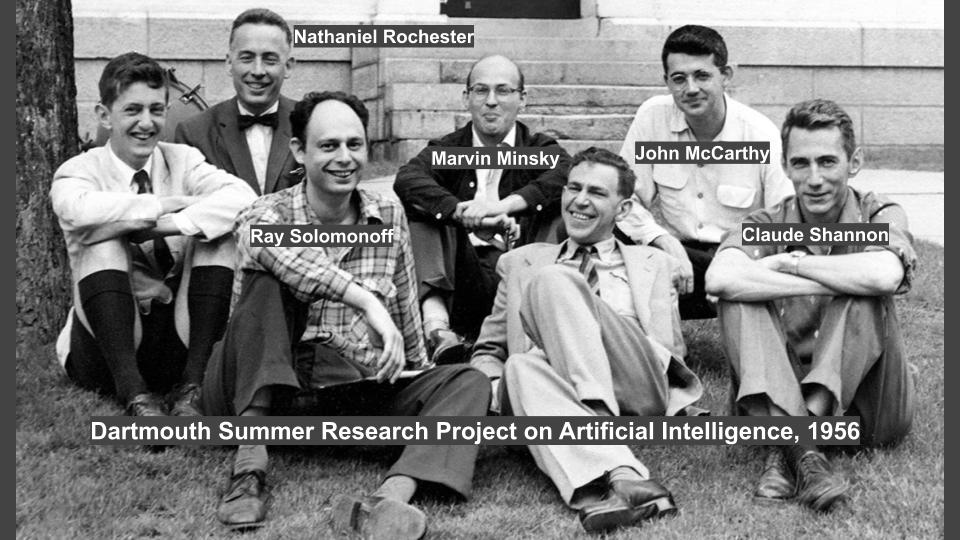
\includegraphics[width=0.9\textwidth]{img/dartmouth-conference.jpg}
      \end{center}
    \end{textblock}

\end{frame}


\begin{frame}
  \note{
    \begin{itemize}
    \item Second phase is made of so-called ``winters'' (periods of lower
      funding or... hype)
    \item However there was still lot of work
    \end{itemize}
  }
  \frametitle{AI winters and expert systems (1973-2000)}

  \begin{textblock}{100}(0,10)
    \begin{center}
      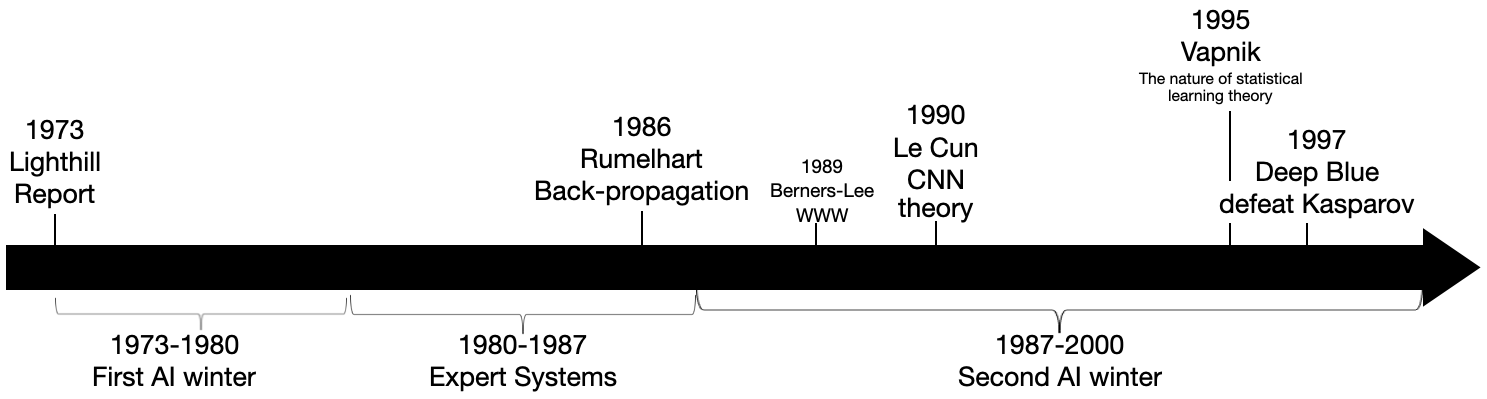
\includegraphics[width=0.95\textwidth]{img/ai_history_1973_2000.png}
    \end{center}
  \end{textblock}

  % Résumé de la frise
  \begin{textblock}{50}(0, 50)
    \begin{itemize}
    \item Lighthill report (1973):
      \begin{itemize}
      \item {\footnotesize ``In no part of the field have the discoveries made so far produced the major impact that was then promised''}
      \item Start of the First Winter
      \end{itemize}
    \item<2-> Proliferation of expert systems (1980s):
      \begin{itemize}
      \item Practical limitations
      \item Start of the Second Winter
      \end{itemize}
    \end{itemize}
  \end{textblock}

  % Enseignements, causes, etc.
  \begin{textblock}{50}(50, 50)
    \begin{itemize}
      \item<3-> Interesting work in the era:
      \begin{itemize}
      \item Technological development: WWW, Python, computing power
      \item Methodological development: statistical learning theory
      \item Deep Blue \vs{} Kasparov
      \item Premise of deep learning
      \end{itemize}
    \end{itemize}
  \end{textblock}

\end{frame}


\begin{frame}
  \note{
    \begin{itemize}
    \item Rise of learning due to work of previous period
    \end{itemize}
  }
  \frametitle{Rise of Machine Learning and Deep Learning (2000-2024)}

  \begin{textblock}{100}(0,10)
    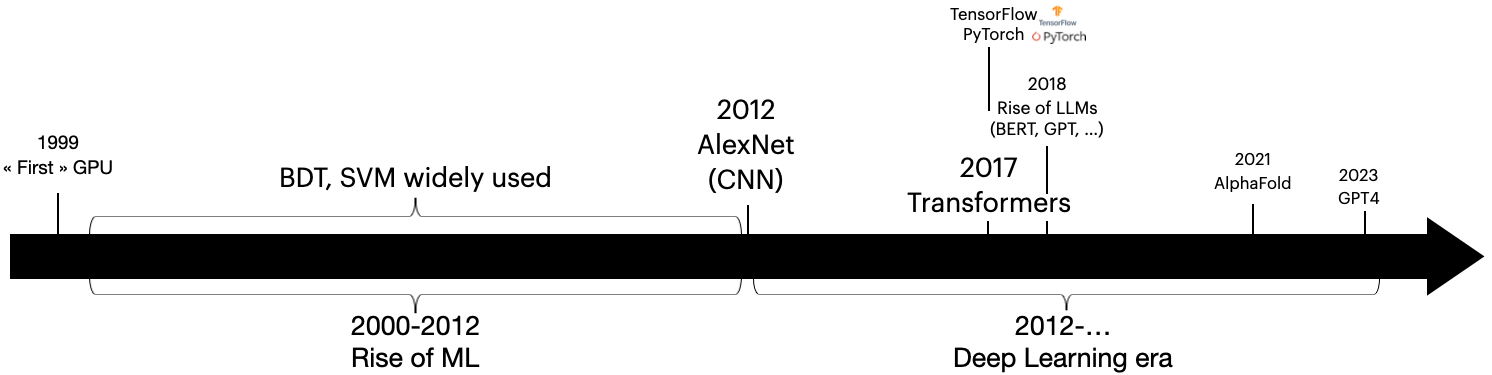
\includegraphics[width=\textwidth]{img/ai_history_2000_2024.png}
  \end{textblock}

  % Commentaire de la frise
  \begin{textblock}{50}(0, 50)
    \begin{itemize}
    \item Rise of \ac{ML} in the early 2000s
    \item<2-> Deep learning era:
      \begin{itemize}
      \item CNN: AlexNet (2012)
      \item Transformers (2017) leads to first LLMs (2018)
      \end{itemize}
    \end{itemize}
  \end{textblock}

  % Enseignements, causes, etc.
  \begin{textblock}{50}(50, 50)
    \onslide<3->{
      \begin{itemize}
      \item Neural networks are mature
      \item Practical causes:
        \begin{itemize}
        \item Lots of data
        \item Processing power (GPU) and storage capability
        \item Mature technology (langages, frameworks)
        \end{itemize}
      \end{itemize}
    }
  \end{textblock}

\end{frame}

\subsection{How to go further?}

\begin{frame}
  \frametitle{General books}

  \nocite{*}

  \begin{block}{AI}<1->
    \printbibliography[heading=none,category=AI]
  \end{block}

  \begin{block}{\ac{ML}}<2->
    \printbibliography[heading=none,category=ML]
  \end{block}
\end{frame}

\begin{frame}
  \frametitle{Deep learning books}

  \nocite{*}

  \printbibliography[heading=none,category=deep_learning]
\end{frame}

\begin{frame}
  \frametitle{Courses \& tutorials}

  \begin{block}{Courses}<1->
    \begin{itemize}
    \item Coursera MOOC:
      \url{https://www.coursera.org/specializations/machine-learning-introduction} (more or less based on \href{https://cs230.stanford.edu/}{Stanford CS230 (Deep Learning)})
    \item FIDLE (Formation Introduction au Deep LEarning): \url{https://fidle.cnrs.fr/}
      (yearly course with practical examples in French)
    \end{itemize}
  \end{block}

  \begin{block}{Challenges}<2->
    \begin{itemize}
    \item Kaggle: \url{https://www.kaggle.com/}
    \item ENS Challenge Data: \url{https://challengedata.ens.fr/}
    \end{itemize}
  \end{block}

  \begin{block}{Tutorials}<3->
    \begin{itemize}
    \item PyTorch tutorials: \url{https://pytorch.org/tutorials/} (in-depth
      tutorials about PyTorch)
    \item scikit-lear tutorials:
      \url{https://scikit-learn.org/stable/user_guide.html} (in depth tutorials
      about scikit-learn)
    \end{itemize}
  \end{block}
\end{frame}
